% !TeX root = ../thuthesis-example.tex

\chapter{模型建立与应用}

\section{使用药材配对直接分析处方效果的尝试}

在引入更复杂的模型前,一个自然的想法是探究参与构成有效处方和不参与的药材配对在基因关联强度上是否有显著差异。如果这种假设成立,我们便可以直接通过评价药方中药材配对的好坏来分析其有效性。对于这一问题,我们可以考察药材配对之间增加的关联边数或者边权重之和,然后将真实的药材配对和所有可能药材配对分别进行排序,作出增益-分位数曲线,从而比较“是否属于已知处方”能否带来统计差异。同时,我们也可以尝试使用基因在药材中通过化合物的定量信息,观察增加这个额外信息相比仅使用STRING给出的分数是否能给出更显著的统计差异。下图是在应用与不应用化合物定量信息的条件下作出的对比曲线:

\begin{figure}[H]
  \centering
  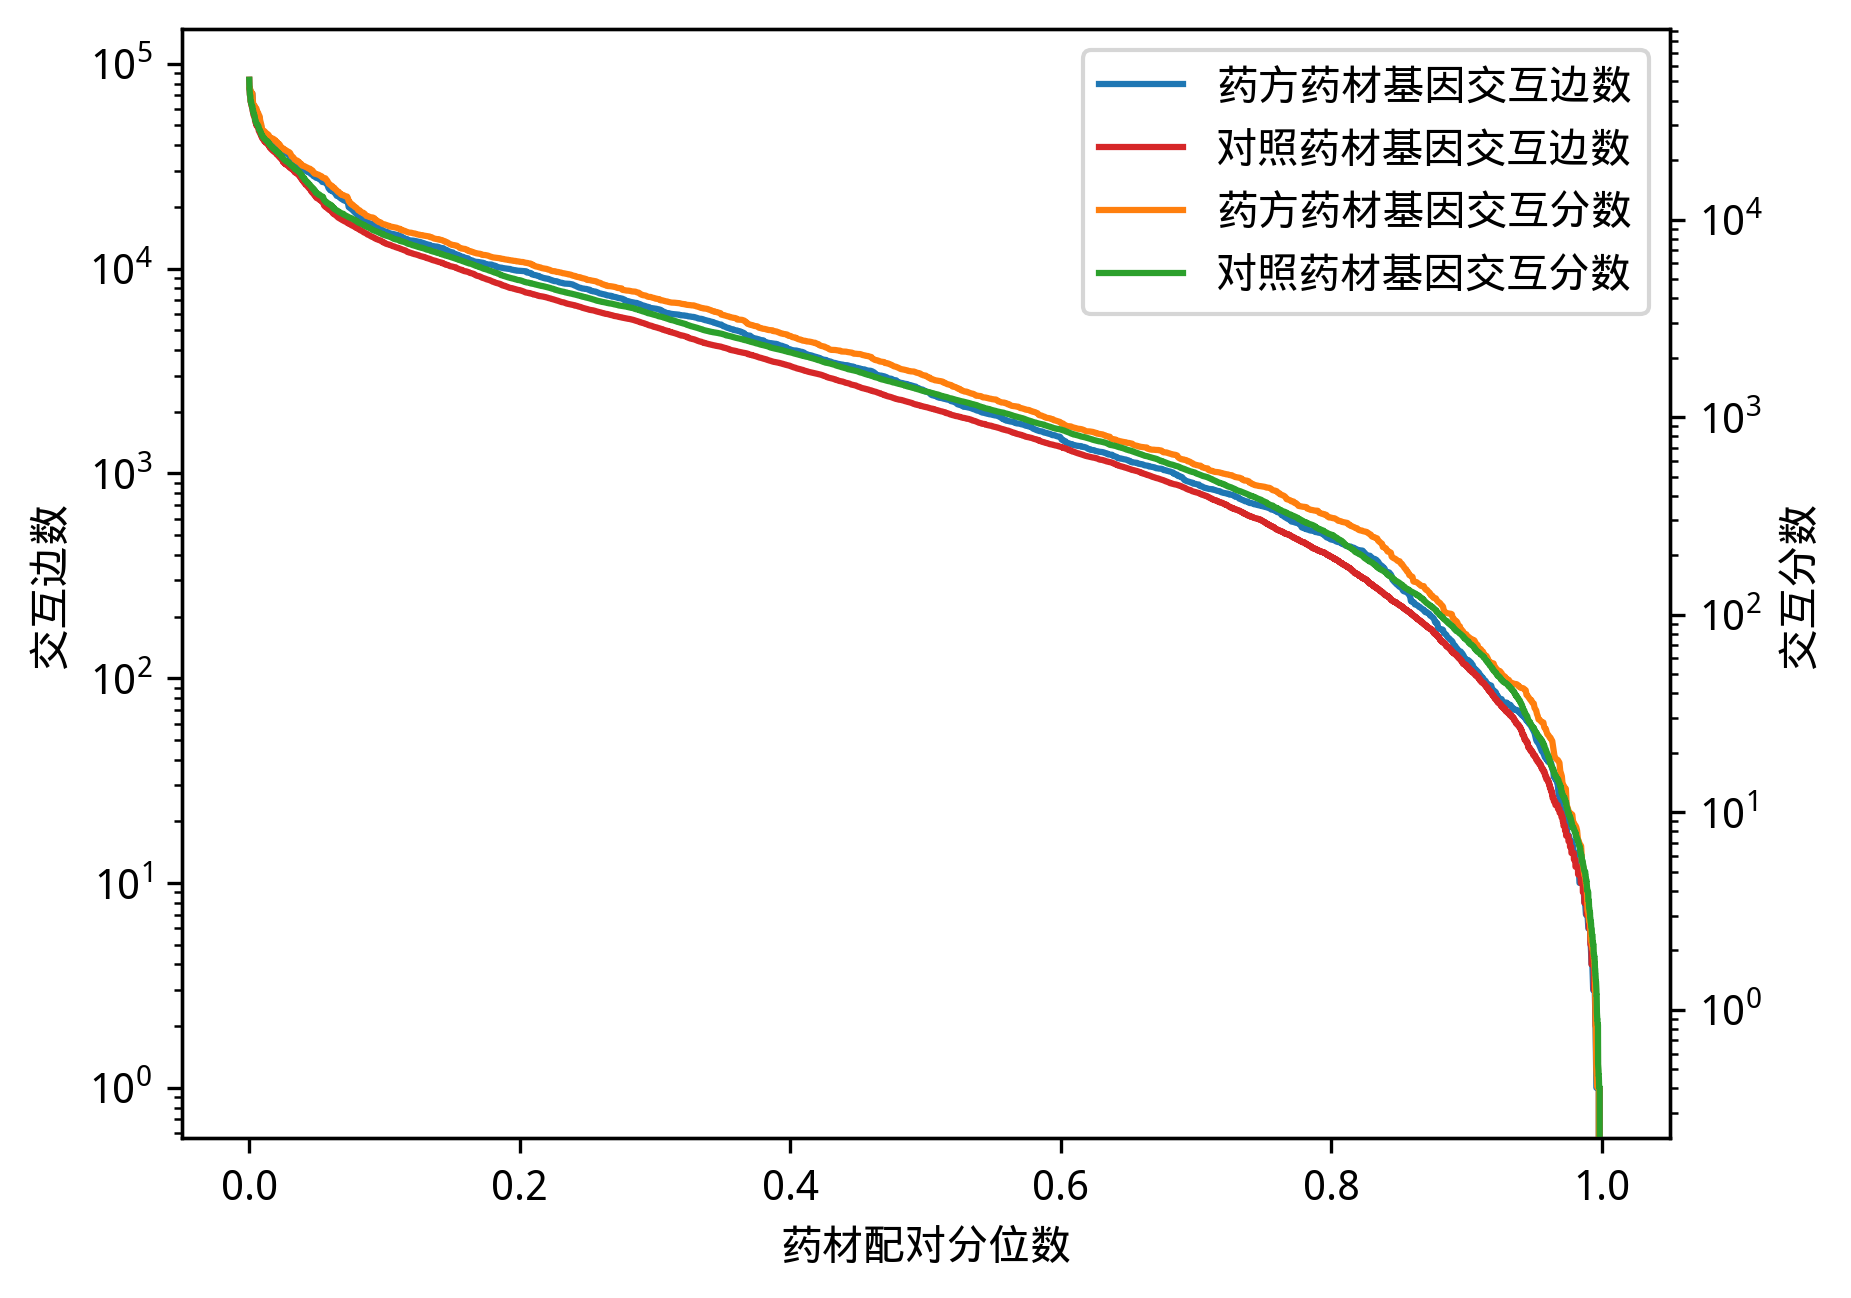
\includegraphics[width=\linewidth]{scores_without_weight.png}
  \caption{不使用化合物定量的药材配对边数/分数增益-分位数曲线}
  \label{fig:score_without_weight}
\end{figure}

\begin{figure}[H]
  \centering
  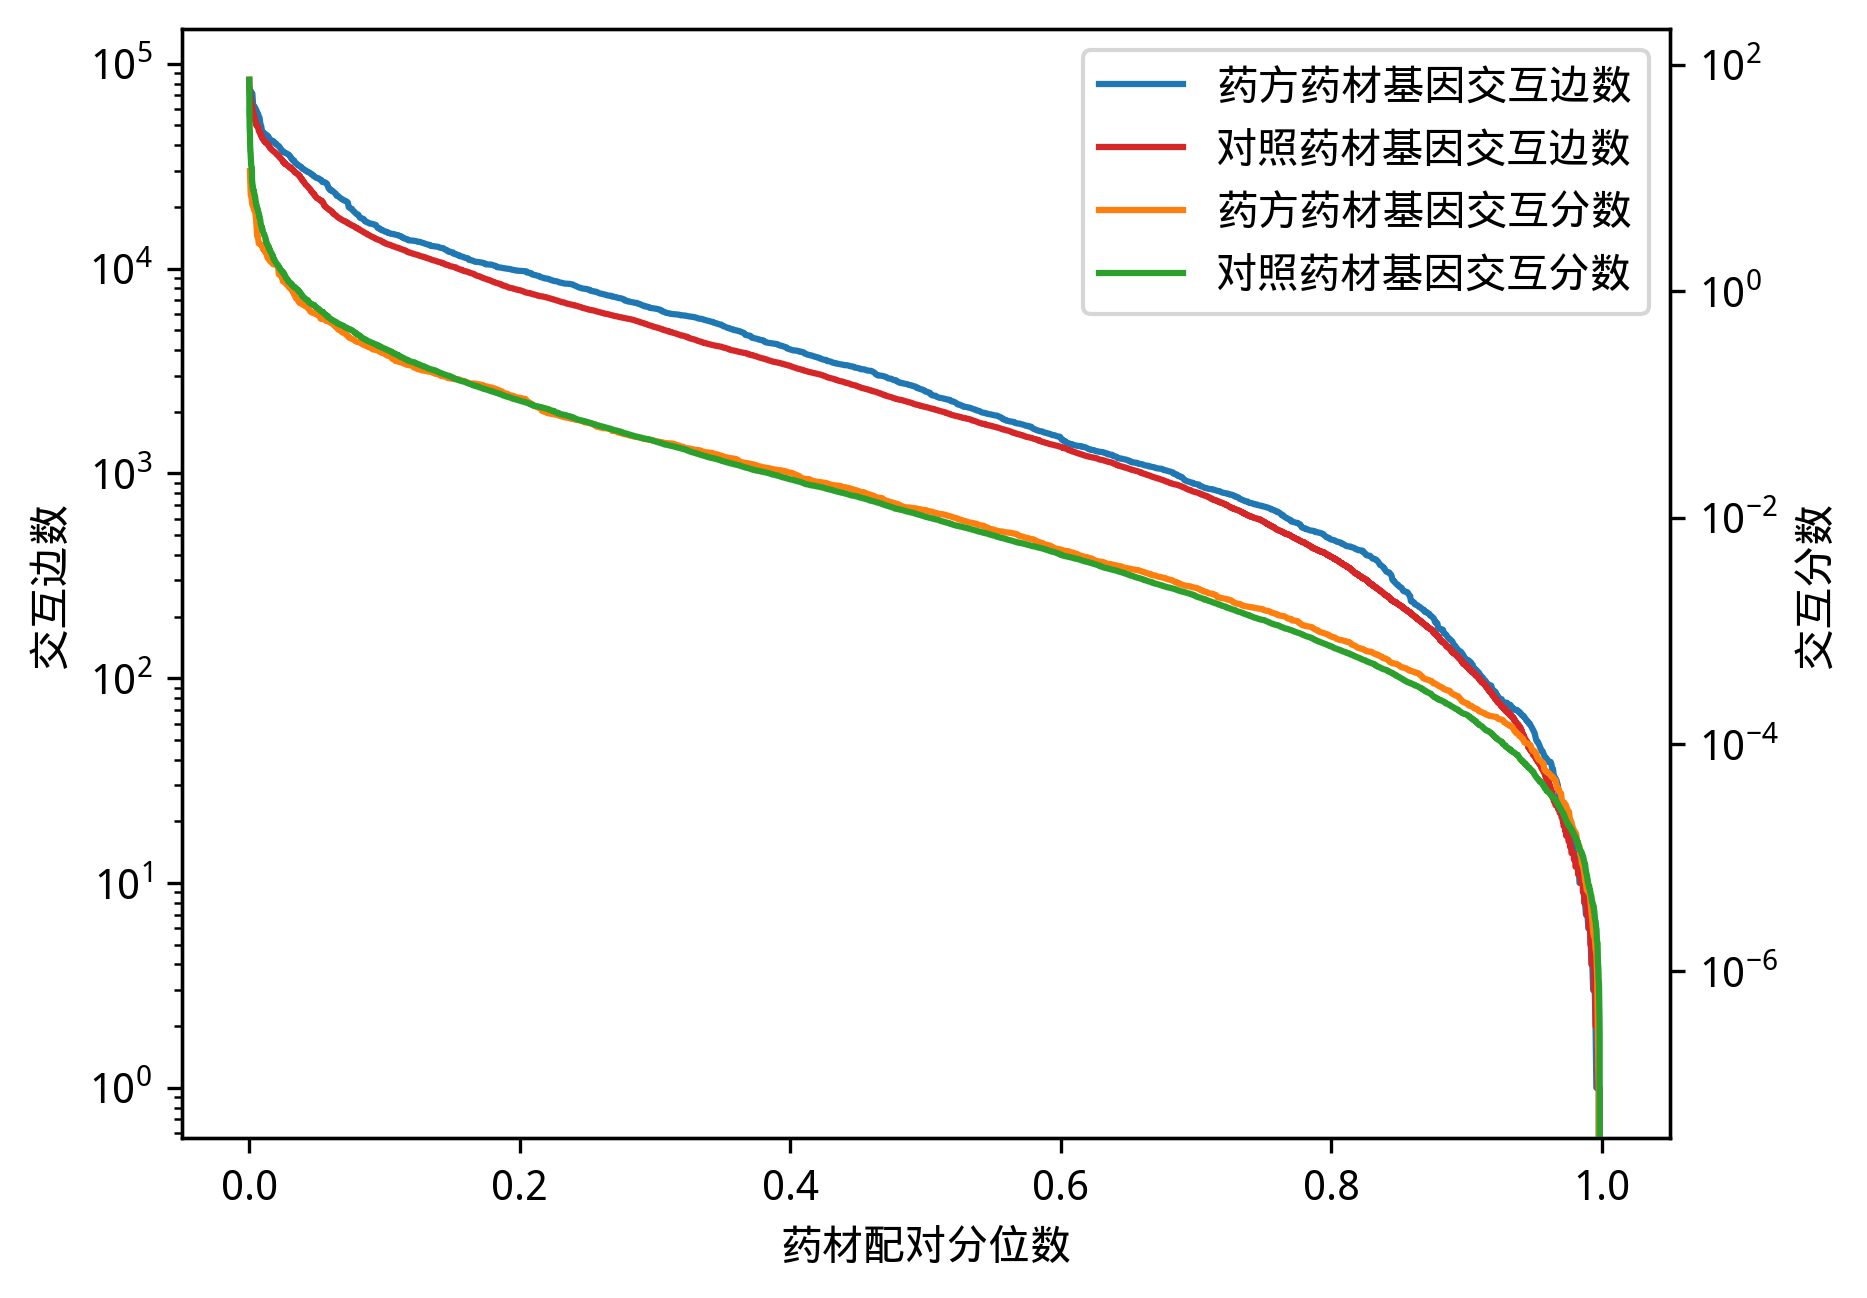
\includegraphics[width=\linewidth]{scores_with_weight.png}
  \caption{使用化合物定量的药材配对边数/分数增益-分位数曲线}
  \label{fig:scores_with_weight}
\end{figure}


虽然我们无法简单地通过边数或分数增益准确地判断药材配对的有效性,但是我们可以从图线中直观地看到,如果不应用化合物定量信息,属于已知处方的药材配对在边数和分数上,几乎各个分位数点处都有优势。使用双样本Kolmogorov-Smirnov检验,可以得到边数的$D$值为$0.0551$,$p$值为$0.00029$, 分数的$D$值为$0.05556$, $p$值为$0.00024$,即这两种指标均能说明是否属于已知药方会导致显著差异,而引入STRING关联分数可以略微提升置信度。

然而,当我们在此引入化合物含量信息后,从图线上发现,增益曲线的差异性几乎消失,甚至有明显的反转区域;双样本Kolmogorov-Smirnov检验的$D$值为$0.0243$,$p$值为$0.35$,无法得到显著差异,这说明化合物含量信息的引入反而使得药材配对的边数和分数增益失去了区分性。这可能是因为化合物含量信息本身存在大量数量级层面的差异,直接相乘引入了过大的噪声。

为了解决上面的问题,我们考虑使用对化合物含量进行归一化,即使用 $\frac{(w_{a1}+w_{a2})(w_{b_1}+w_{b2})}{w_{a1}w_{b2}+w_{b1}w_{a2}}$来作为 $1, 2$ 两个药材中基因对 $(a, b)$ 的化合物定量权重。这样,我们可以得到如下的增益曲线:

\begin{figure}[H]
  \centering
  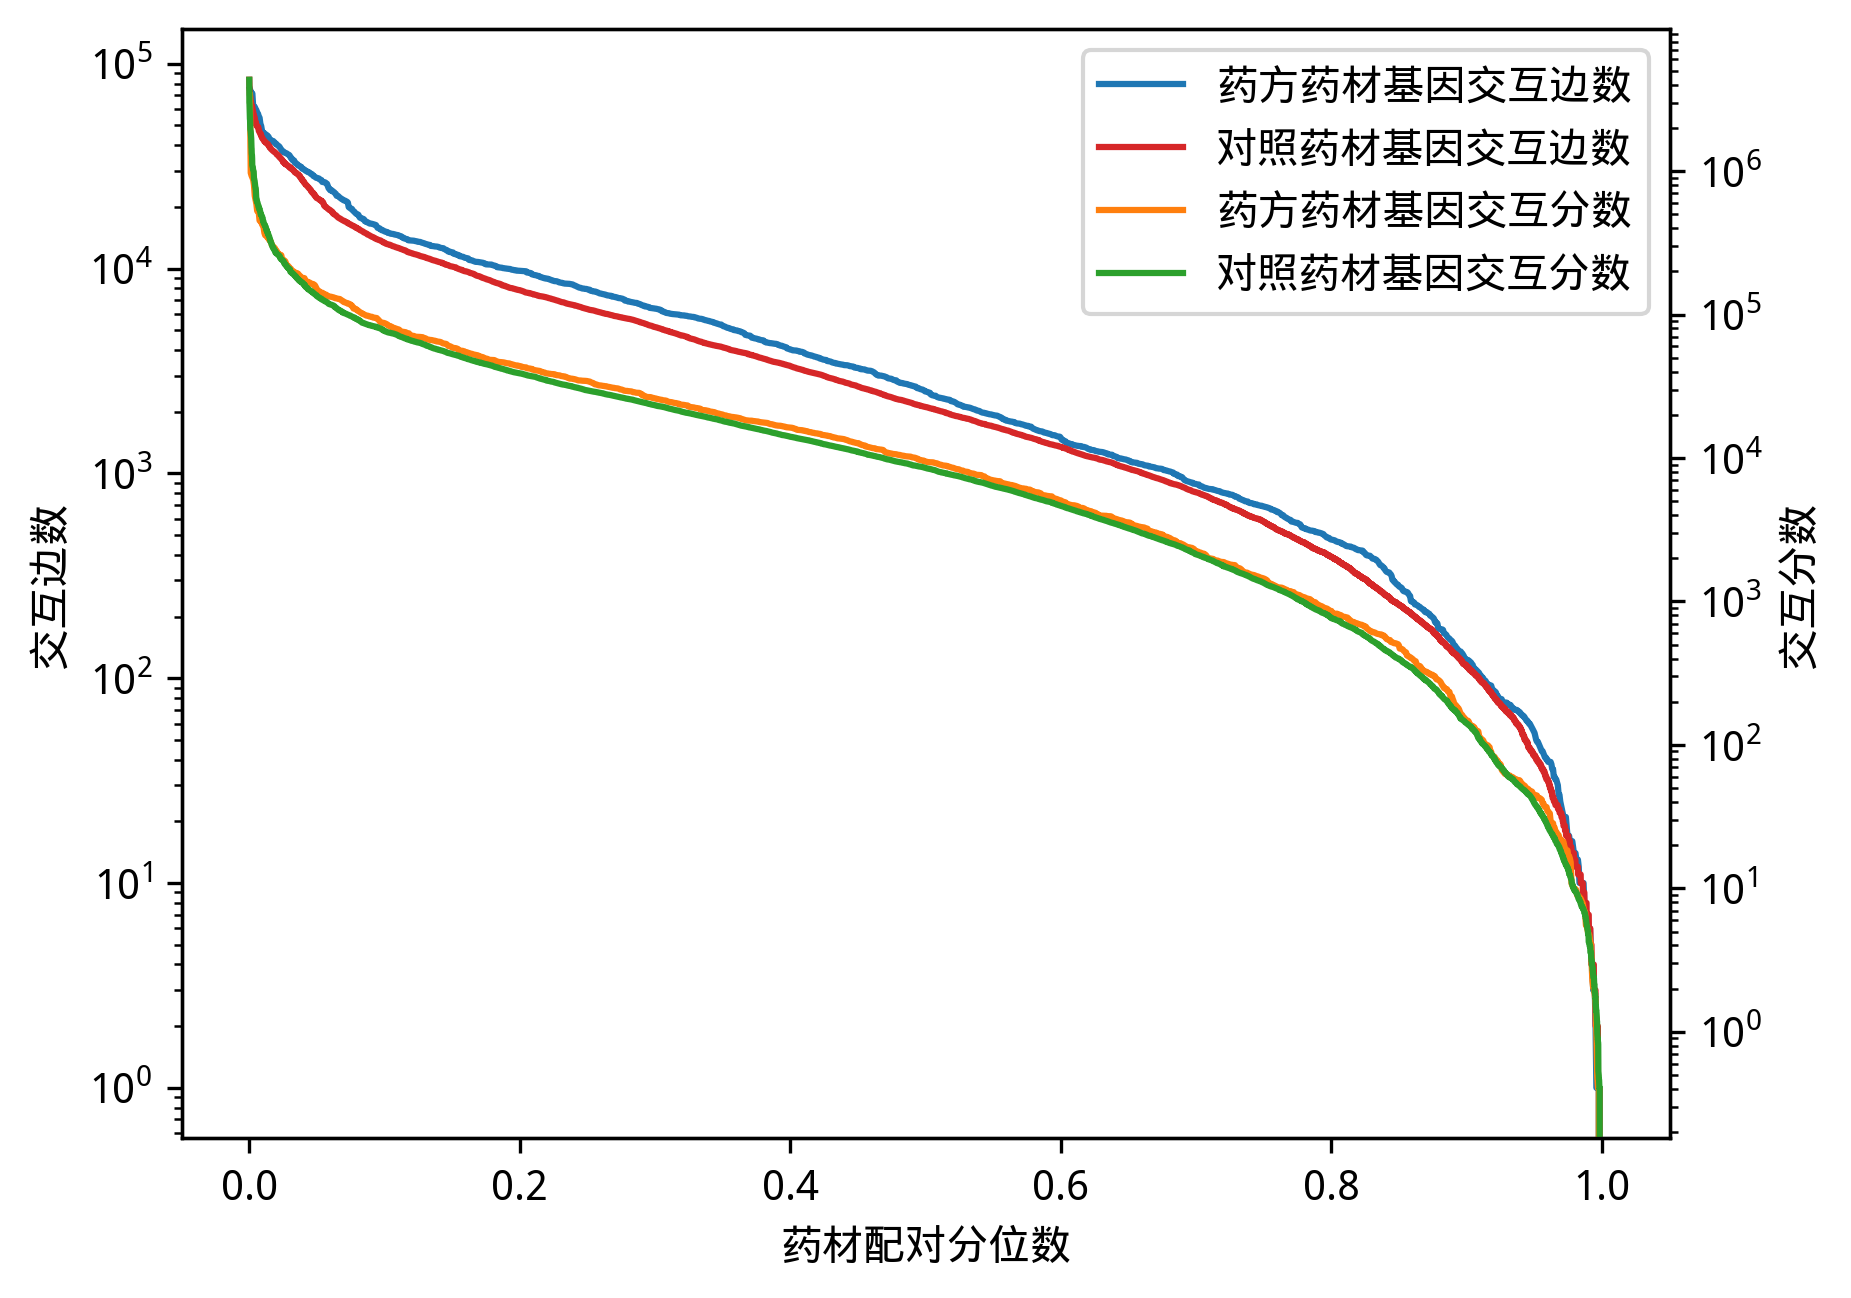
\includegraphics[width=\linewidth]{scores_with_normalized_weight.png}
  \caption{使用归一化化合物定量的药材配对边数/分数增益-分位数曲线}
  \label{fig:scores_with_normalized_weight}
\end{figure}

这里的图线相比之前得到了改善,可以观察出药方药材配对几乎始终在对照药材配对上方,但双样本Kolmogorov-Smirnov检验具有$D$值为$0.0314$,$p$值为$0.11$,仍然没有显著性,说明对数在此问题中可能是一个更好的转换方式。但定量信息依然没有为药材配对的边数和分数增益带来提升,说明我们还需要建立更复杂的模型来运用定量信息解释处方的效果。

% edge
% KstestResult(statistic=0.05506882248177303, pvalue=0.0002908647549561178, statistic_location=5799, statistic_sign=-1)
% unweighted
% KstestResult(statistic=0.05564546832511763, pvalue=0.00024155665548500303, statistic_location=3674.2729999999983, statistic_sign=-1)
% weighted
% KstestResult(statistic=0.024379685069236018, pvalue=0.34918573567118794, statistic_location=0.0013520617904999987, statistic_sign=-1)
% normalized
% KstestResult(statistic=0.031446876287792414, pvalue=0.11124597693644322, statistic_location=13623.52746273345, statistic_sign=-1)

\section{基于图神经网络的处方效果预测}

如果从处方层面考虑问题,我们可以作出这样的假设:各基因受处方整体的作用等于处方中各药材影响的代数和,来自不同药材或不同化合物的基因影响在混同后是完全等价的。在这种假设下,我们可以直接遍历处方中的每个药材求和,得到每个基因的总表达影响,这样就把一个处方建模成了一系列以基因作为顶点,从化合物含量信息推出的总表达影响为点权重,基因之间的关联为边,STRING分数为边权重的图。利用图神经网络的方法,我们便可以训练模型对处方的效果进行预测,其中设《中国药典》中已经存在的处方为正例,而随机生成的、大概率不会有现实药理作用的处方为负例,便形成了一个通过图特征进行二分类的问题。在这里,我们首先考虑朴素的图卷积网络(GCN),它使用简单的层次化方法聚合节点的邻域信息,适合于这里的基因表达关联。

在实际的训练和预测过程中,一方面,图的节点数,即处方中的药材数,会显著影响连接密度和图表示,是重要的特征,但有效处方的实际大小存在如下显著的分别:

\begin{figure}[H]
  \centering
  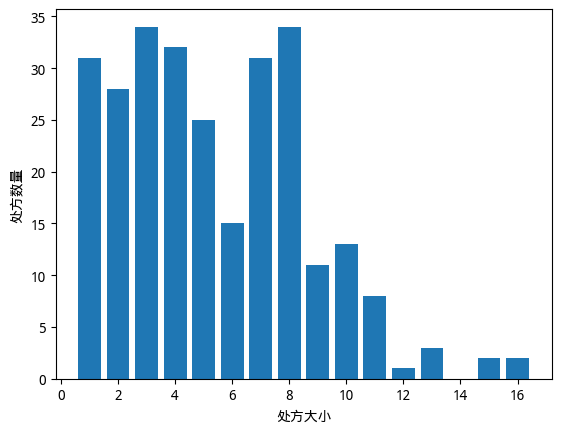
\includegraphics[width=\linewidth]{prescription_size.png}
  \caption{《中国药典》中药材均在ccTCM中收录的处方大小分布}
  \label{fig:prescription_size}
\end{figure}

为了防止GCN学习到的实际上是有效处方较可能拥有的大小而非底层的关联信息,我们不能简单地随机指定生成虚拟药方的大小,而要使生成集合中各大小的处方比例也与《中国药典》中的已知处方相近。

另一方面,由于正例是固定的,数量上非常有限,而负例可以几乎无限地任意生成,因此相比于构造平衡的数据集,我们更倾向于采样更多负例来训练。在这里,我们尝试使用$1:9$的正负例比,并通过基于交叉熵损失函数的训练来优化模型。得到的训练-验证曲线如下:
